\section{Das erste Deformationslemma}

\begin{definition}[Riemannsche Metrik]
    Eine \textit{Riemannsche Metrik} $g$ ist ein Skalarprodukt 
    \[ g_p:T_pM \times T_pM \to \R \]
    für jeden Punkt $p$, sodass für alle Vektorfelder $X$ und $Y$ die Abbildung 
    $p \to g_p(X(p), Y(p))$ glatt ist.
    Wir schreiben 
    \[ g_p(x, y) = \langle x, y \rangle \]
\end{definition}

\begin{definition}[Gradient]
    Es sei $M$ \textit{Riemannsche Mannigfaltigkeit}, also eine Mannigfaltigkeit
    zusammen mit einer Riemannschen Metrik $g$. Außerdem sei $f: M \to \R$ glatt.
    Dann ist der \textit{Gradient} von $f$ das (einzigartige) 
    Vektorfeld $\grad f$ für das gilt:
    \[ \langle X, \grad f \rangle = \opd fX \]
\end{definition}

Falls $M$ eine Riemannsche Mannigfaltigkeit, $f: M \to \R$ glatt, ist $p \in M$ 
ein kritischer Punkt von $f$ genau dann, wenn $\grad f (p) = 0$. 

Man kann auf jeder Mannigfaltigkeit eine Riemannsche Metrik definieren.

\begin{figure}[H]
    \centering
    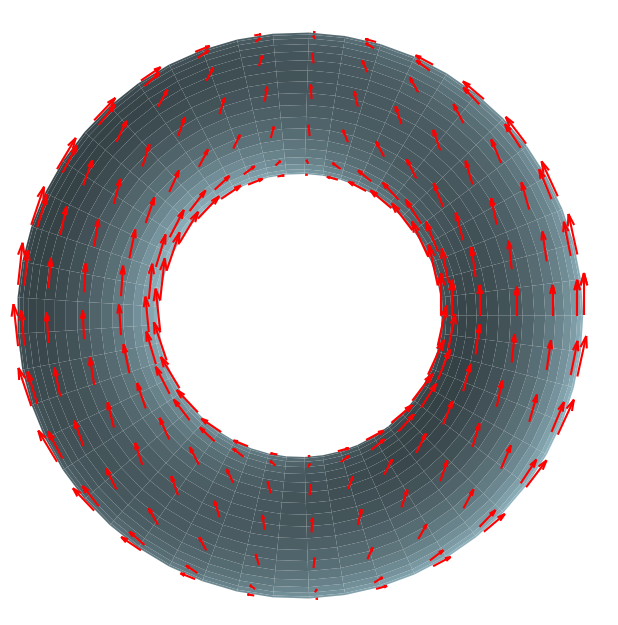
\includegraphics[width=0.7\linewidth]{resources/Me-Diagram4-gradient-of-hightmapping.png}
    \label{fig:me-diagram4}
    \caption{Gradient der Höhenfunktion auf dem Torus}
\end{figure}

\begin{definition}[Flusslinie, Wang]
    Es sei $X$ ein Vektorfeld auf einer glatten Mannigfaltigkeit $M$. Für einen
    glatten Weg $\gamma: I \to M$, $I \subseteq \R$ ein Intervall, 
    definiere für $t_0 \in I$:
    \[ \derive[\gamma]{t}(t_0) = \opd \gamma (t_0) \left(\derive{t}\right) \in T_{\gamma(t_0)}M \]
    wobei $\derive{t} \in T_pM$ das durch die Identität auf $\R$
    induzierte Element im Tangentialraum ist.
    Ein Weg $\gamma: I \to \R$ heißt \textit{Flusslinie} eines Vektorfeldes $X$,
    falls für alle $t_0 \in I$ gilt:
    \[ X(\gamma(t_0)) = \derive[\gamma]{t}(t_0) \]
\end{definition}

\begin{definition}[1-Parameter Gruppe aus Diffeomorphismen]
    Eine \textit{1-Parameter Gruppe aus Diffeomorphismen} ist eine glatte 
    Abbildung
    \[ \varphi: \R \times M \to M \text{, wobei } (t, p) \mapsto \varphi_t(p) \]
    Sodass für alle $s$, $t \in \R$ gilt:
    \[ \varphi_{t + s} = \varphi_t \circ \varphi_s \]
    und 
    \[ \varphi_0 = \id_M \]
    Ich schreibe:
    \[ \varphi_{\bullet}(p): \R \to M ; t \mapsto \varphi_t(p) \]
    Wir sagen eine 1-Parameter Gruppe aus Diffeomorphismen wird von einem
    Vektorfeld $X$ generiert, falls für alle $p \in M$ gilt
    \[ X(p) = \derive[\varphi_{\bullet}(p)]{t}(0) \]
\end{definition}

Ist $\varphi$ eine 1-Parameter Gruppe aus Diffeomorphismern, so ist für alle 
$t \in \R$ $\varphi_t$ ein Diffeomorphismus mit Inverse $\varphi_{-t}$.

Bemerke: Falls $X$ eine 1-Parameter Gruppe aus Diffeomorphismen $\varphi$ erzeugt,
dann ist für alle $p \in M$ der Weg $\varphi_{\bullet}(p)$ eine Flusslinien von $X$, denn
\begin{align*}
    X(\varphi_{t_0}(p)) 
    & = \derive[\varphi_{\bullet}(\varphi_{t_0}(p))]{t}(0)
    = T_0 \varphi_{\bullet}(\varphi_{t_0}(p)) \left(\derive{t}\right) \\
    & = T_0 \varphi_{t_0 + \bullet}(p) \left(\derive{t}\right)
    = T_{t_0} \varphi_{\bullet}(p) \cdot T_0 (t_0 + \id_{\R}) \left(\derive{t}\right) \\
    & = T_{t_0} \varphi_{\bullet}(p) \left(\derive{t}\right)
    = T_{t_0} \varphi_{\bullet}(p) \left(\derive{t}\right) \\
    & = \derive[\varphi_{\bullet}(p)]{t}(t_0)
\end{align*}

\begin{lemma}
    \label{lemma:generierende vektorfelder}
    Es sei $X$ ein Vektorfeld auf einer glatten Mannigfaltigkeit $M$ mit kompaktem 
    Träger. Dann generiert $X$ eine eindeutige 1-Parameter Gruppe aus 
    Diffeomorphismen.
\end{lemma}

\begin{proof} Der Beweis ist recht umfangreich, wird hier aber ausgelassen. \end{proof}

\begin{theorem}[Erstes Deformationslemma]
    \label{theorem:erstes deformationslemma}
    Es sei $M$ eine glatte Mannigfaltigkeit und $f: M \rightarrow \R$ eine
    glatte Abbildung. Hat $f$ keine kritischen Werte im Intervall $[a, b]$ und 
    ist $f^{-1}[a, b]$ kompakt, so existiert ein Diffeomorphismus 
    $M^a \rightarrow M^b$, und $M^a$ ist ein Deformationsretrakt von $M^b$.
\end{theorem}

Das ist genau die erste Aussage, die wir schon am Anfang beim Torus beobachtet 
haben!

Die Idee des Beweises ist es, $M^a$ entlang der Richtung, in die $f$ am stärksten
steigt, also entlang des Gradientenfeldes mit einem Diffeomorphismus $\varphi$ 
"nach oben zu ziehen", bis $\varphi(f^{-1}(a)) = f^{-1}(b)$.

\begin{proof}[Beweis erstes Deformationslemma]
    Es existiert eine kompakte Umgebung $K \in M$ von $f^{-1}[a, b]$. Dies folgt
    aus Whitneys Einbettungssatz und dem Satz von Heine-Borel.
    Sei $\rho: M \to \R$ eine glatte, positive Funktion, sodass
    \[ \rho(p) = 1 / \langle \grad f, \grad f \rangle \]
    für alle $p \in f^{-1}[a, b]$ und die außerhalb von $K$ verschwindet und für
    die für alle $p \in K$, die keine kritischen Punkte sind, gilt: 
    \[ 0 \leq \rho(p) \leq 1 / \langle \grad f, \grad f \rangle \]
    Bemerke dass $\rho$ innerhalb von $f^{-1}[a, b]$ wohldefiniert 
    ist, da sich keine kritischen Punkte im Intervall $[a, b]$ befinden. 
    Definiere ein Vektorfeld $X$ durch
    \[ X(p) = \rho(p) \cdot \grad f (p) \]
    Dann hat $X$ kompakten Träger, erfüllt also die Vorraussetzungen von 
    Lemma~\ref{lemma:generierende vektorfelder}. Sei also $\varphi$ die
    einzigartige 1-Parameter Gruppe aus Diffeomorphismen, die von $X$ generiert
    wird. 
    Wir bekommen für jedes $p \in M$ eine Abbildung 
    $f \circ \varphi_{\bullet}(p): \R \to \R$.
    
    \proofheading{Behauptung 1} Für alle $p \in M$, $t_0 \in \R$ und $q = \varphi_{t_0}(q)$
    ist $\derive{t} f \circ \varphi_{\bullet}(p) (t_0) \in [0, 1]$ und falls $f(\varphi_t(q)) \in [a, b]$
    gilt sogar $\derive{t} f \circ \varphi_{\bullet}(q) (t_0) = 1$.

    Für $q = \varphi_{t_0}(p)$:
    \begin{align*}
        \derive{t} f \circ \varphi_{t_0}(p)
        & = T_{\varphi_{t_0}(p)} f \cdot T_{t_0}\varphi_{\bullet}(p) \left( \derive{t} \right)
        = \opd f (q) \cdot X(q) \\
        & = \langle X(q), \grad f (q) \rangle 
        = \rho(q) \langle \grad f (q), \grad f (q) \rangle \in [0, 1]
    \end{align*}
    
    $f \circ \varphi_{\bullet}(p)$ ist also monoton wachsend für alle $p \in M$.

    Falls sogar $f(\varphi_p(t_0)) \in [a, b]$, dann gilt
    \[ \frac{d}{dt} f \circ \varphi^p (t_0) = 1 \]
    \sectiondone

    \proofheading{Behauptung 2} Für $p \in f^{-1}(a)$, $t_0 \in [0, b-a]$ gilt $f(\varphi_{t_0}(p)) \in [a, b]$.
    
    \[ f(\varphi_{t_0}(p)) \geq f(\varphi_0(p)) = a \]
    und
    \begin{align*}
        f(\varphi_t(p)) 
        & \leq f(\varphi_{b-a}(p)) \\
        & = \int_0^{b-a}\derive{t} f(\varphi_t(p)) \opd t + f(\varphi_0(p)) \\
        & = \int_0^{b-a}\rho(\varphi_t(p)) \langle \grad f (\varphi_t(p)), \grad f (\varphi_t(p)) \rangle \opd t + a \\
        & \leq \int_0^{b-a} 1 \, \opd t + a \\
        & = b
    \end{align*}
    \sectiondone

    \proofheading{Behauptung 3} Unter $\varphi_{b-a}$ wird die Niveaumenge 
    $f^{-1}(a)$ auf die Niveaumenge $f^{-1}(b)$ abgebildet.
     
    Für $p \in f^{-1}(a)$ gilt:
    \[ \varphi_{a-a}(p) = \varphi_0(p) = p \]
    und für $t_0 \in [0, b - a]$ gilt wegen Behauptung 1 und 2
    \[ \derive{t}f(\varphi_{\id_{\R} - a}(p)) (t_0) = 1 \]
    also
    \[ f(\varphi_{b - a}(p)) = f(\varphi_{0}(p)) + (b - a) = b \]
    Genauso gilt für $q \in f^{-1}(b)$: $f(\varphi_{a - b}(q)) = a$, also 
    $\varphi_{b - a}(f^{-1}(a)) = f^{-1}(b)$.
    \sectiondone

    \proofheading{Behauptung 4} $\varphi_{b - a} (M^a) = M^b$

    "$\subseteq$": Sei $p \in M^a$. OBdA. existiert $s \in [0, b-a]$, sodass 
    $f(\varphi_s(p)) = a$, ansonsten gilt für alle 
    $s \in [0, b-a]: f(\varphi_s(p)) \leq a < b$. Dann gilt
    \[ f(\varphi_{b-a}(p)) \leq f(\varphi_{b-a+s}(p)) = f(\varphi_{b-a}(\varphi_s(p))) = b \] 
    "$\supseteq$": Analog.
    \sectiondone

    Damit ist $\left. \varphi_{b-a} \right\vert_{M^a}$ ein Diffeomorphismus zwischen
    $M^a$ und $M^b$. 

    Betrachte nun $r: M^b \times \R \to M^b$,
    \[  
        r(p, t) = \begin{cases}
            p & \text{ falls } f(p) \leq a \\
            \varphi_{t(a - f(p))}(p) & \text{ falls } a \leq f(p) \leq b 
        \end{cases}
    \]

    Dann ist $r$ stetig, $r(\cdot, 0)$ ist die Identität auf $M^b$, 
    $r(\cdot, 1)|_{M^a}$ ist die Identität auf $M^a$ und 
    $r(1, M^b) \subseteq M^a$, also ist $M^a$ ein Deformationsretrakt von $M^b$.

\end{proof}

\begin{corollary}
    Es sei $M$ eine Mannigfaltigkeit, $f: M \to \R$ eine glatte Funktion ohne
    kritische Werte in $[a, b]$. dann ist $f^{-1}[a, b]$ diffeomorph zu den
    Mannigfaltigkeiten mit Rand $f^{-1}(a) \times [a, b]$ und 
    $f^{-1}(b) \times [a, b]$.
\end{corollary}
